\chapter{Grundlagen}

In diesem Kapitel wird das Wissen vermittelt, welches benötigt wird um zu Verstehen, wie \acp{NNUE} im Rahmen von Schachcomputern funktionieren. Zuerst wird die Evaluation, wie sie in herkömmlichen Schachcomputern funktioniert erklärt, auch \ac{HCE} genannt.

\section{Hand-crafted Evaluation}
\label{chap:HCE}

Die Evaluation einer Schachposition ist eine heuristische Methode der Position einen numerischen Wert zuzuordnen. Hätten wir unendliche Ressourcen könnten wir aus jeder Position alle mögliche Zugfolgen sehen und der Positionen einer der drei Werte: -1 (Verlust), 0 (remis), 1 (Gewinn) geben. In der Realität ist es nicht möglich den exakten Wert der Stellung zu kennen, deshalb wird in der \ac{HCE} versucht anhand von Menschen festgelegten Kriterien einen Wert der Position zuzuordnen. 
Vor der Verbreitung von \acp{NN}, war \ac{HCE} die einzige Form der Positions-Evaluation. 

\section{Neuronale Netze}

\tikzset{
  every neuron/.style={
    circle,
    draw,
    minimum size=1cm
  },
  neuron missing/.style={
    draw=none, 
    scale=4,
    text height=0.333cm,
    execute at begin node=\color{black}$\vdots$
  },
}

\begin{figure}
  % taken from: https://tex.stackexchange.com/questions/153957/drawing-neural-network-with-tikz
  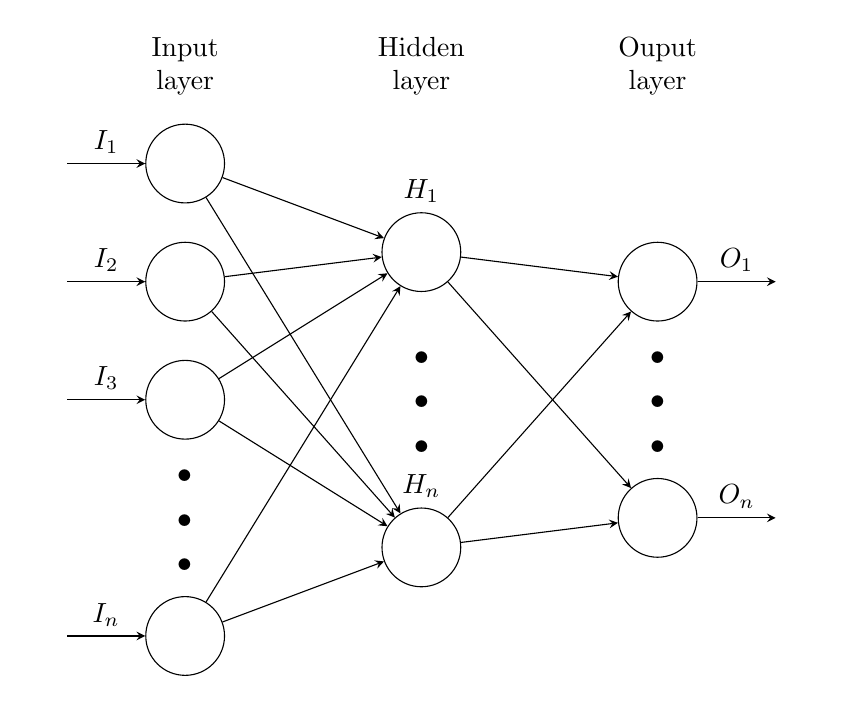
\begin{tikzpicture}[x=1.5cm, y=1.5cm, >=stealth]
  
  \foreach \m/\l [count=\y] in {1,2,3,missing,4}
    \node [every neuron/.try, neuron \m/.try] (input-\m) at (0,2.5-\y) {};
  
  \foreach \m [count=\y] in {1,missing,2}
    \node [every neuron/.try, neuron \m/.try ] (hidden-\m) at (2,2-\y*1.25) {};
  
  \foreach \m [count=\y] in {1,missing,2}
    \node [every neuron/.try, neuron \m/.try ] (output-\m) at (4,1.5-\y) {};
  
  \foreach \l [count=\i] in {1,2,3,n}
    \draw [<-] (input-\i) -- ++(-1,0)
      node [above, midway] {$I_\l$};
  
  \foreach \l [count=\i] in {1,n}
    \node [above] at (hidden-\i.north) {$H_\l$};
  
  \foreach \l [count=\i] in {1,n}
    \draw [->] (output-\i) -- ++(1,0)
      node [above, midway] {$O_\l$};
  
  \foreach \i in {1,...,4}
    \foreach \j in {1,...,2}
      \draw [->] (input-\i) -- (hidden-\j);
  
  \foreach \i in {1,...,2}
    \foreach \j in {1,...,2}
      \draw [->] (hidden-\i) -- (output-\j);
  
  \foreach \l [count=\x from 0] in {Input, Hidden, Ouput}
    \node [align=center, above] at (\x*2,2) {\l \\ layer};
  
  \end{tikzpicture}
  \caption{Ein exemplarisches \acl{NN}}
  \label{grundlagen:beispiel-nn}
\end{figure}

\Acp{KNN} oder einfach \acp{NN} genannt, sind Computer Systeme, die dem biologischen Vorbild des Gehirns nachempfunden sind. In Abbildung \autoref{grundlagen:beispiel-nn} ist ein einfaches \acl{NN} zu sehen. Es besteht aus 

\ac{NN} bestehen aus

\subsection{Das Neuron}

% neuronen wie sie im nerfen systems eines menschen vorhanden sind
Das Neuron ist der elementare Bestandteil eines \acp{NN}.
Um Neuronen eines \acp{NN} zu verstehen, schauen wi

\subsection{Backpropagation}
% viel muss man davon nicht kennen, da pytorch das übernimmt (automatic through automatic differentiation)

\subsection{Convolutional Neural Networks}
% kann vl entfernt werden (schau am ende ob man es noch braucht (seiten))
% nur ein kurzer exkurs da es in andern neuronalen netzen für schach computer verwendet wird


\subsection{Loss funcntions}


\subsection{Quantization}

\section{SIMD}

\ac{SIMD}

\subsection{Memory Alignment}

